\chapter{VAE Evaluation Studies}
\label{chap:8_vae_evaluation_studies}
In this section, we will evaluate the the performance of our VAE model in regards to its reconstruction ability. We aim to explore the effects of the different modifications to the reward function, as presented in \cref{subsec:5_vae_reconstruction}. To do this, we will begin with a plain reconstruction error, before adding a depth weighting, and finally edge loss.
Moreover, we explore these implementations to both MSE and BCE loss.

For each of the models, we assess its training and test curves, then visualise its reconstruction for a set of test images.
An overview of the models and their time-to-train is shown below:
\begin{table}[hbt]
    \centering
    \begin{tabular}{||c|c|c|c||}
    \hline
        ID & Model & Epoch & Time \\
    \hline\hline
        1 & Vanilla MSE & 40 & 19h 4m \\\hline
        2 & Vanilla BCE & 50 & 1d 14h 36m \\\hline
        3 & Depth Weighted MSE & 100 & 3d 4h 52m \\\hline
        4 & Depth Weighted BCE & 60 &  1d 13h 54m \\\hline
        5 & Depth Weighted MSE with Edge Loss & 60 & 1d 22h 49m \\\hline
        6 & Depth Weighted BCE with Edge Loss & 100 & 3d 3h 37m \\
    \hline
    \end{tabular}
    \caption{List of VAE models.}
    \label{tab:8_all_vae_models}
\end{table}

\section{Vanilla Loss Function}
\label{sec:8_vanilla}
Beginning first with the vanilla reconstruction loss, the overall loss function for a batch $B$ of $m$ of samples is: 
\begin{equation}
    \widetilde{\loss}_B\,(\boldsymbol{\theta}, \boldsymbol{\phi}; \d^{(i)}, {\d^f}^{(i)} ) =
    \frac{1}{m} \sum_{i=1}^m
    \Bigg(
    \log \pbt ({\d^f}^{(i)} |\, \bz^{(i,l)}) 
    -
    \DKL{\qbp(\bz |\, \d^{(i)})}{\log \pbt(\bz)}
    \Bigg)
    \label{eq:8_vanilla_loss_estimator_batch}
\end{equation}
Then, the reconstruction loss $\loss^{(i)}_{\text{REC}} = \log \pbt (\boldsymbol{\hat{d}^f}^{(i)} |\, \bz^{(i,l)})$ can be replaced with the vanilla MSE and BCE, which is implemented in practice as:
\begin{equation}
    \loss^{(i)}_{\text{MSE}} = \norm{\, \boldsymbol{\hat{d}^f}^{(i)} - \boldsymbol{d^f}^{(i)}}
    \label{eq:8_mse_vanilla_loss}
\end{equation}
\begin{equation}
    \loss^{(i)}_{\text{BCE}} =\boldsymbol{d^f}^{(i)} \log \sigmoid{\boldsymbol{\hat{d}^f}^{(i)}} +  (1 - \boldsymbol{d^f}^{(i)}) \log \sigmoid{1 - \boldsymbol{\hat{d}^f}^{(i)}}
    \label{eq:8_bce_vanilla_loss}
\end{equation}
where $\sigma$ is used to denote the \textit{sigmoid} activation function.

\subsection{Training}
We train our network on 202,558 depth images for 100 epochs. Their training and validation plots are shown below:
\begin{figure}[htb]
    \centering
    \begin{subfigure}[b]{\textwidth}
        \centering
        \captionsetup{justification=centering}
        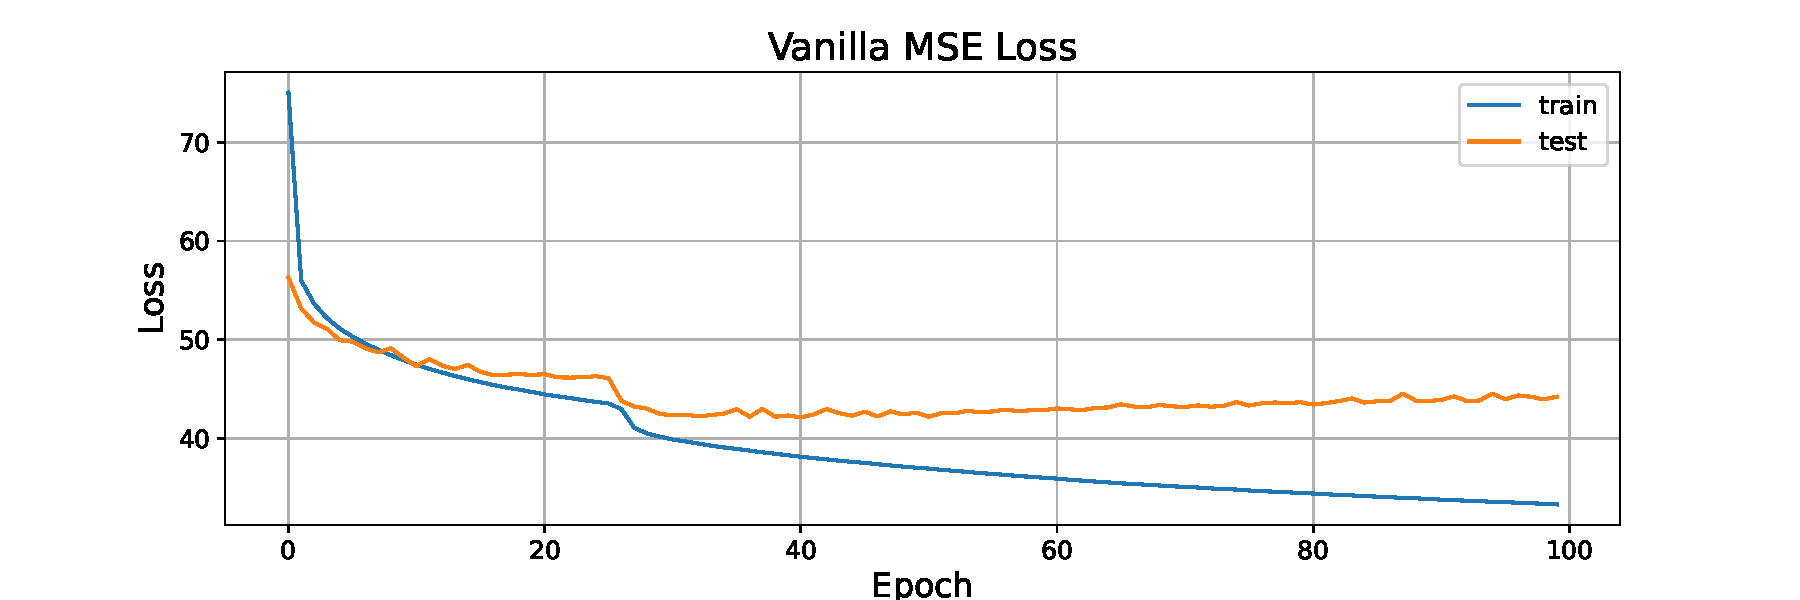
\includegraphics[width=0.99\textwidth]{figures/8_/1_final_MSE_plain.pdf}
        \label{fig:1_final_MSE_plain}
    \end{subfigure} \\
    \begin{subfigure}[b]{\textwidth}
        \centering
        \captionsetup{justification=centering}
        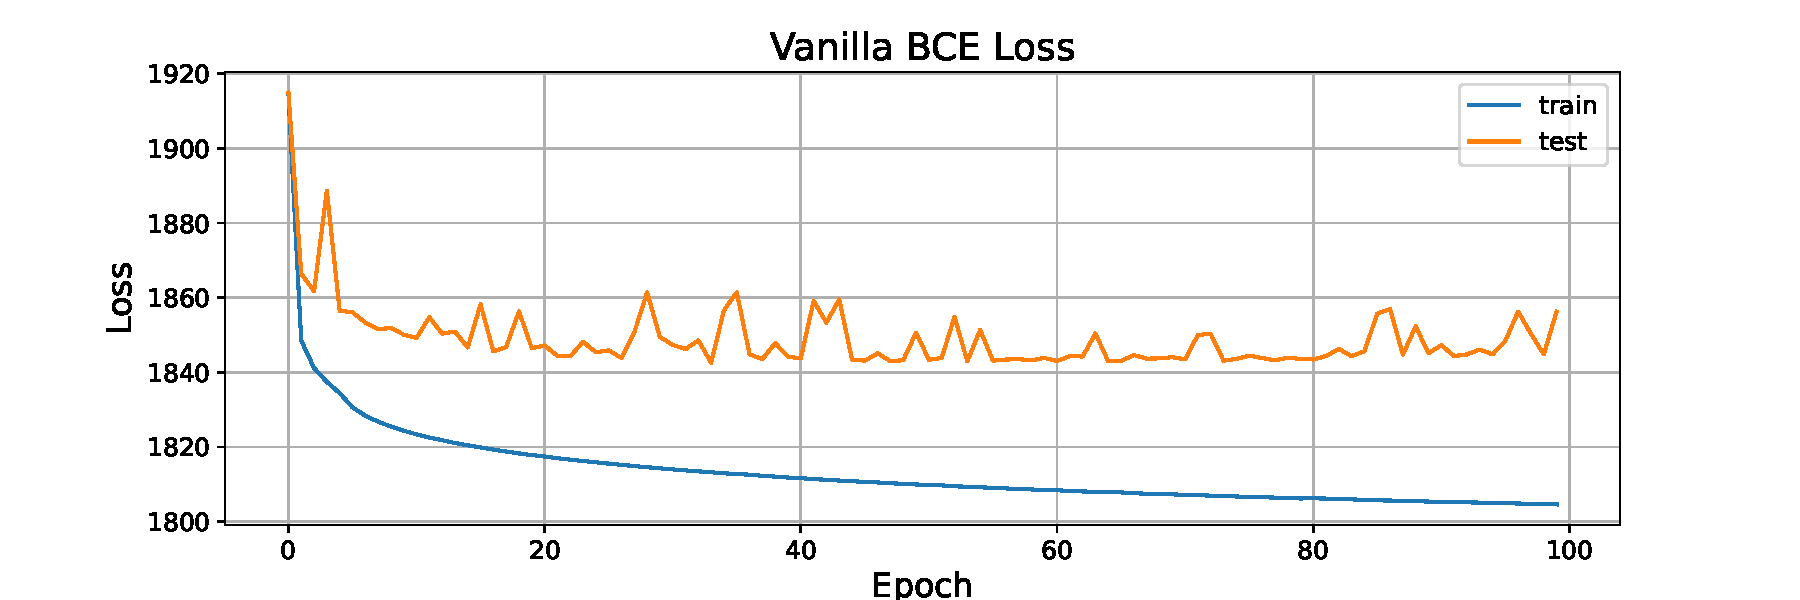
\includegraphics[width=0.99\textwidth]{figures/8_/4_final_BCE_plain.pdf}
        \label{fig:4_final_BCE_plain}
    \end{subfigure} 
    \caption{Training and test loss for the vanilla MSE and BCE models.}
    \label{fig:8_vanilla_vae}
\end{figure}

\subsection{Testing}





\section{Depth Weighted Loss}
\label{sec:8_depth}
One of the adverse effects of these two additions is the excessive blurring of the depth images. Since we specified that it was important to \textit{at least} detect close obstacles, the VAE was inclined to create very large obstacles, or even \textit{phantom obstacles}. This occurred because the VAE only incurred a high loss if it \textit{did not} detect a close obstacle, but not if it misdetected one. 
\begin{equation}
    \loss^{(i)}_{\text{MSE}} = \norm{\, \boldsymbol{\hat{d}^f}^{(i)} - \boldsymbol{d^f}^{(i)}}
    \label{eq:8_mse_depth_weighted_loss}
\end{equation}
\begin{equation}
    \loss^{(i)}_{\text{BCE}} =\boldsymbol{d^f}^{(i)} \log \sigmoid{\boldsymbol{\hat{d}^f}^{(i)}} +  (1 - \boldsymbol{d^f}^{(i)}) \log \sigmoid{1 - \boldsymbol{\hat{d}^f}^{(i)}}
    \label{eq:8_bce_depth_weighted_loss}
\end{equation}


\subsection{Training}

\begin{figure}[htb]
    \centering
    \begin{subfigure}[b]{\textwidth}
        \centering
        \captionsetup{justification=centering}
        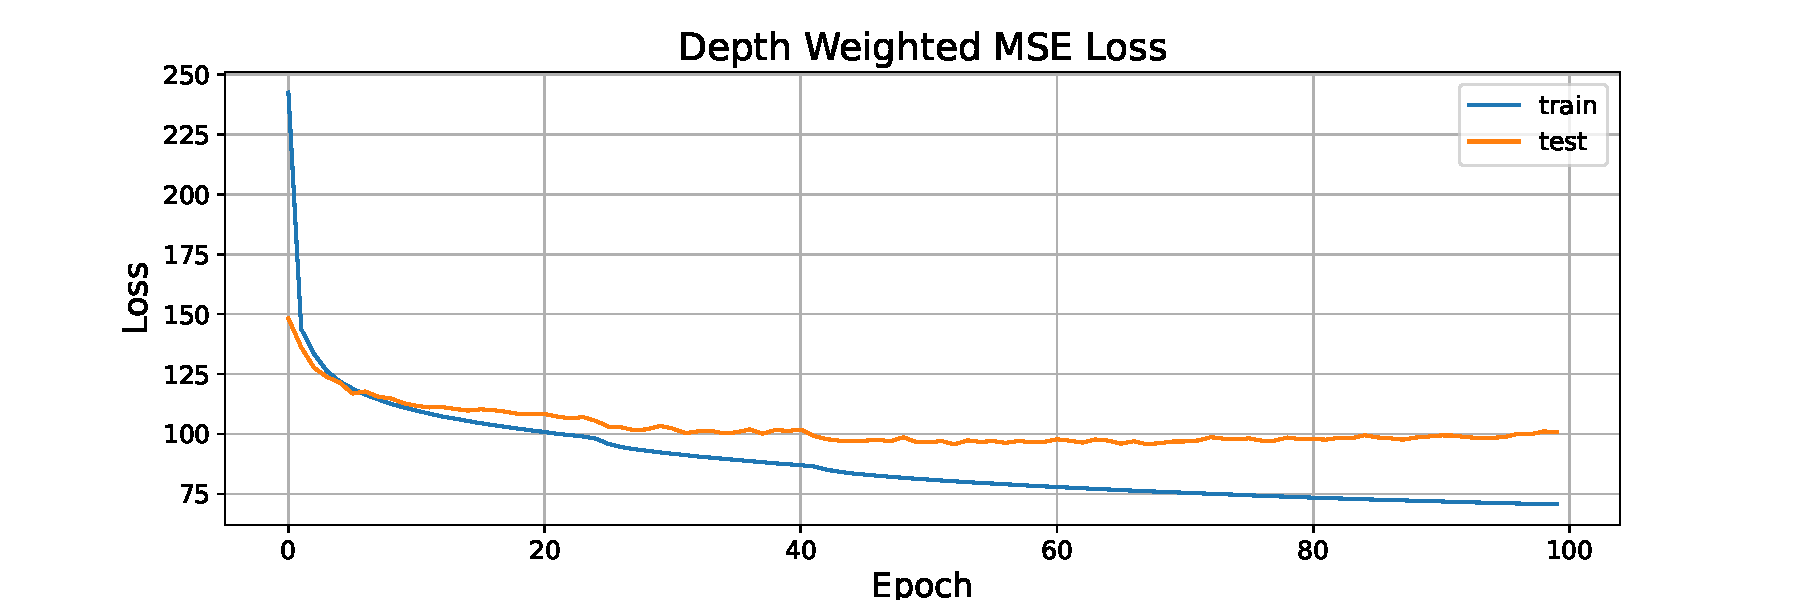
\includegraphics[width=0.99\textwidth]{figures/8_/2_final_MSE_depth_weighted10.pdf}
        \label{fig:2_final_MSE_depth_weighted10}
    \end{subfigure} \\
    \begin{subfigure}[b]{\textwidth}
        \centering
        \captionsetup{justification=centering}
        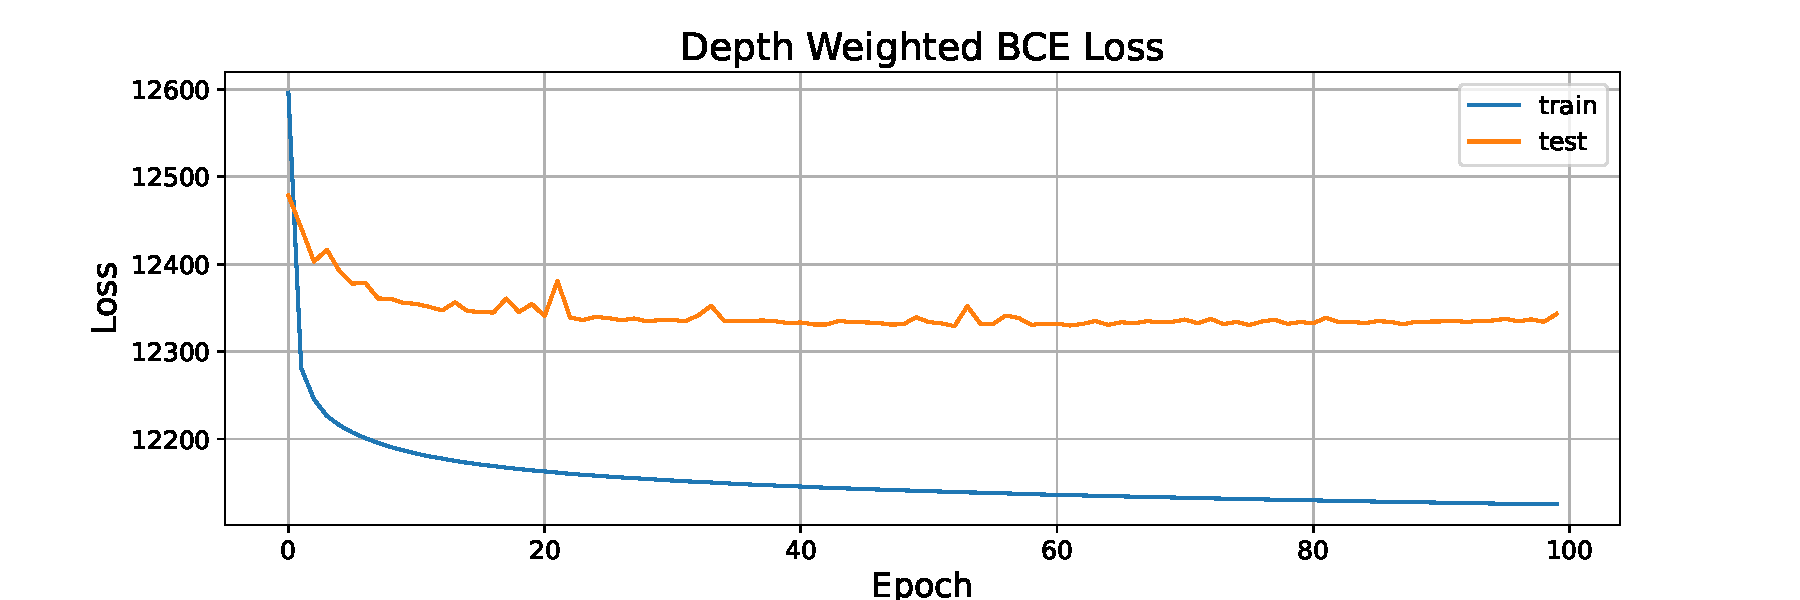
\includegraphics[width=0.99\textwidth]{figures/8_/5_final_BCE_depth_weighted10.pdf}
        \label{fig:5_final_BCE_depth_weighted10}
    \end{subfigure} 
    \caption{Training and test loss for the depth weighted MSE and BCE models.}
    \label{fig:8_depth_vae}
\end{figure}



\section{Depth Weighted Loss With Edge Loss}
\label{sec:8_edge_depth}
the edge loss aims to improve the resolution (contrast) of the reconstructions, so that they are not over-blurred as a result of filtering. In a sense, it provides an extra loss signal to give the VAE a direction on how to filter depth images implicitly.

\subsection{Training}

\begin{figure}[htb]
    \centering
    \begin{subfigure}[b]{\textwidth}
        \centering
        \captionsetup{justification=centering}
        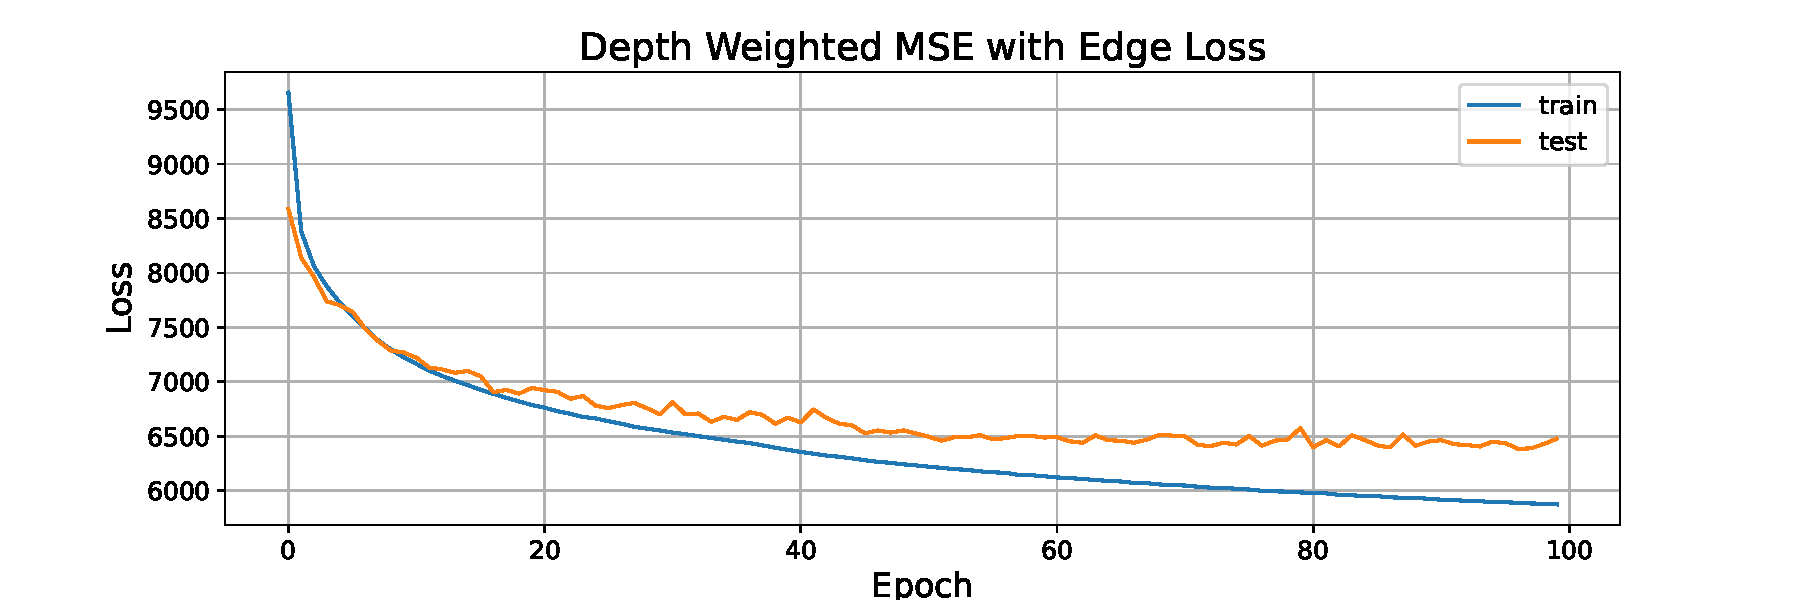
\includegraphics[width=0.99\textwidth]{figures/8_/3_final_MSE_depth_weighted10_with_depth_weighted_canny_edge_mae100_loss.pdf}
        \label{fig:3_final_MSE_depth_weighted10_with_depth_weighted_canny_edge_mae100_loss}
    \end{subfigure} \\
    \begin{subfigure}[b]{\textwidth}
        \centering
        \captionsetup{justification=centering}
        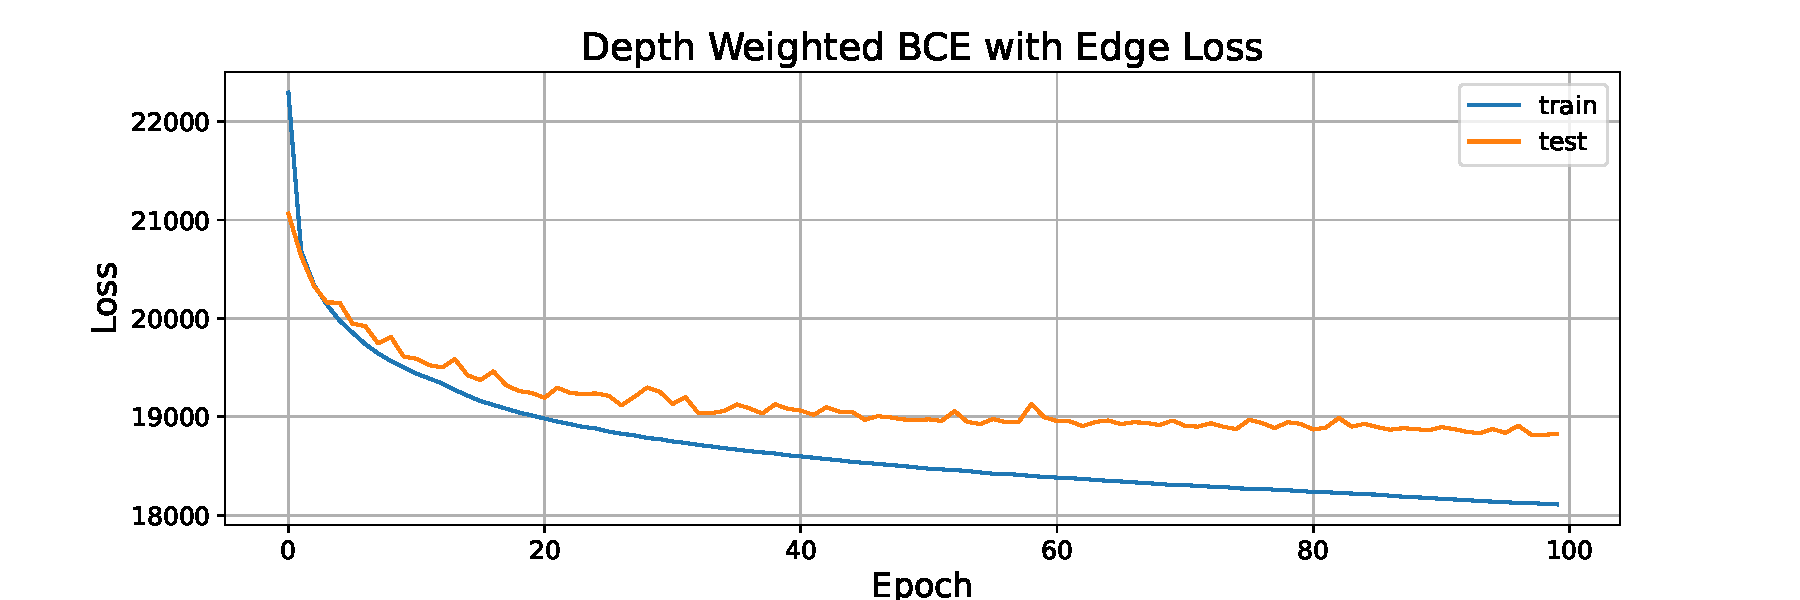
\includegraphics[width=0.99\textwidth]{figures/8_/6_final_BCE_depth_weighted10_with_depth_weighted_canny_edge_mae100_loss.pdf}
        \label{fig:6_final_BCE_depth_weighted10_with_depth_weighted_canny_edge_mae100_loss}
    \end{subfigure} 
    \caption{Training and test loss for the depth weighted MSE and BCE models when adding an edge loss term.}
    \label{fig:8_edge_depth_weighted_vae}
\end{figure}

